\documentclass{article}

\usepackage{amsmath}
\usepackage{amssymb}
\usepackage{float}
\usepackage{tikz}
\usepackage{xcolor}


\usepackage[utf8]{inputenc}
\usepackage[T1]{fontenc}

% \usepackage[polish]{babel}

\usepackage{listings}
\lstset{
    language=SQL,
    inputencoding=utf8x,
    extendedchars=\true,
    literate={ą}{{\k{a}}}1
             {Ą}{{\k{A}}}1
             {ę}{{\k{e}}}1
             {Ę}{{\k{E}}}1
             {ó}{{\'o}}1
             {Ó}{{\'O}}1
             {ś}{{\'s}}1
             {Ś}{{\'S}}1
             {ł}{{\l{}}}1
             {Ł}{{\L{}}}1
             {ż}{{\.z}}1
             {Ż}{{\.Z}}1
             {ź}{{\'z}}1
             {Ź}{{\'Z}}1
             {ć}{{\'c}}1
             {Ć}{{\'C}}1
             {ń}{{\'n}}1
             {Ń}{{\'N}}1
}

\newcommand\hlight[1]{\tikz[overlay, remember picture,baseline=-\the\dimexpr\fontdimen22\textfont2\relax]\node[rectangle,fill=blue!50,rounded corners,fill opacity = 0.2,draw,thick,text opacity =1] {$#1$};}

\title{Działania na macierzach}
\date{2026}

\begin{document}
\maketitle

%%%%%%%%%%%%%%%%%%%%%%%%%%%%%%%%%%%%%%%%%%%%%%%%%%%%%%%%%%%%%%%%
\section{Dodawanie Macierzy}
%===============================================================
\subsection{Definicja}
Macierze $A=[a_{ij}]$ oraz $B=[b_{ij}]$ wymiar $m \times n$.
Ich sumą/różnicą nazywamy macierz $C=A \pm B=[c_{ij}]$, również wymiaru 
$m \times n$, której elementy są określone jako:
$$
    c_{ij} = a_{ij} \pm b_{ij}, \text{gdzie:}\,i = 1,2, \dots, m,\,j=1,2,\dots,n
$$
%===============================================================
\subsection{Własności}
Macierze $A, B$ wymiaru $m \times n$:
\begin{itemize}
    \item $A + B = B + A$
    \item $(A + B) + C = A + (B + C)$
    \item $A + \mathbf{0} = \mathbf{0} + A = A$
    \item $A + (-A) = \mathbf{0}$
    \item $\alpha(A+B) = \alpha A + \alpha B$, gdzie $\alpha \in \mathbb{C}$
    \item $(\alpha + \beta)A = \alpha A + \beta B$, gdzie $\alpha, \beta \in \mathbb{C}$
    \item $(\alpha \beta)A = \alpha(\beta A)$, gdzie $\alpha,\beta \in \mathbb{C}$
\end{itemize}

%%%%%%%%%%%%%%%%%%%%%%%%%%%%%%%%%%%%%%%%%%%%%%%%%%%%%%%%%%%%%%%%
\section{Mnożenie Macierzy}
%===============================================================
\subsection{Definicja}
Macierz $A = [a_{ij}]$ wymiaru $m \times n$, macierz $B=[b_{ij}]$
wymiaru $n \times k$.
Iloczynem macierzy $A$ i $B$ nazywamy macierz $C = A \cdot B = [c_{ij}]$,
wymiaru $m \times k$, której elementy sa określone jako:
$$
    c_{ij} = a_{i1}b_{1j}+a_{i2}b_{2j}+ \dots +a_{in}b_{nj} = \sum_{l=1}^{n}{a_{il}b_{lj}}
$$
Element $c_{ij}$ jest zatem sumą kolejnych iloczynów $i$-tego 
wiersza macierzy $A$, oraz $j$-tej kolumny macierzy $B$.
%===============================================================
\subsection{Własności}
Macierz $A = [a_{ij}]$ wymiaru $m \times n$, macierz $B=[b_{ij}]$
wymiaru $n \times k$:
\begin{itemize}
    \item $A(B+C) = AB + AC$
    \item $(A+B)C = AC + BC$
    \item $A(\alpha B) = (\alpha A)B = \alpha AB$
    \item $(AB)C = A(BC) = ABC$
    \item $AI_{n} = I_{m}A = A$
\end{itemize}

%%%%%%%%%%%%%%%%%%%%%%%%%%%%%%%%%%%%%%%%%%%%%%%%%%%%%%%%%%%%%%%%
\section{Transpozycja}
%===============================================================
\subsection{Definicja}
Macierz $A = [a_{ij}]$ wymiaru $m \times n$.
Macierzą transponowaną do macierzy $A$ nazywamy macierz $B=[b_{ij}]$
wymiaru $n \times m$, której elementy są określone jako:
$$
    b_{ij} = a_{ji}, \, \text{gdzie: } i = 1,2, \dots , n,\,
    j=1,2, \dots, m
$$
Oznacza to, że w macierzy transponowanej zamieniamy wiersze na kolumny.

Macierz transponowaną do $A$ oznaczamy $A^{T}$.
%===============================================================
\subsection{Własności}
Macierz $A = [a_{ij}]$ wymiaru $m \times n$, macierz $B$ odpowiedniego
rozmiaru.
\begin{itemize}
    \item $(A+B)^{T} = A^{T} + B^{T}$
    \item $(AB)^{T} = B^{T}A^{T}$
    \item $(A^{T})^{T} = A$
    \item $(\alpha A)^{T} = \alpha A^{T}$
    \item $(A^{k})^{T} = (A^{T})^{k}$
\end{itemize}

%%%%%%%%%%%%%%%%%%%%%%%%%%%%%%%%%%%%%%%%%%%%%%%%%%%%%%%%%%%%%%%%
\section{Wyznacznik}
Istnieje kilka definicji wyznacznika macierzy, tutaj zostanie 
podana tzw. permutacyjna definicja wyznacznika. 
%===============================================================
\subsection{Definicja}
Wyznacznikiem macierzy $A = [a_{ij}]$ wymiaru $n \times n$ nazywamy
wyrażenie:
$$
    |A| = \sum_{\mathbb{Z}}{sgn(i_{1},i_{2},\dots,i_{n})
        a_{1i_{1}}a_{1i_{2}}\cdots a_{1i_{n}}}
$$
gdzie:
\begin{itemize}
    \item $(i_{1},i_{2},\dots,i_{n})$ - dowolna permutacja,
    \item $\mathbb{Z}$ - zbiór wszystkich permutacji.
\end{itemize}

Można zauważyć, że wyznacznik jest wielomianem $n^{2}$ zmiennych,
zawierających $n!$ składników (jednomianów stopnia $n$).

%===============================================================
\subsection{Interpretacja geometryczna wyznacznika}
Wyznacznik w przypadku $n=2$ można traktować jako pole powierzchni
równoległoboku, tworzonego przez wektory będące kolumnami macierzy:
$$
    A = 
    \begin{bmatrix} a & c \\ b & d \end{bmatrix}
    =
    \begin{bmatrix} \vec{u} & \vec{v} \end{bmatrix}
$$
gdzie:
\begin{itemize}
    \item $\vec{u}$ - wektor o długości $u$ i kącie nachylenia $\alpha$,
    \item $\vec{v}$ - wektor o długości $v$ i kącie nachylenia $\beta$.
\end{itemize}
Zatem:
$$
    \begin{array}{ll}
        a = u \cos(\alpha) & b = u \cos(\alpha)\\
        c = v \cos(\beta) & d = v \cos(\beta)
    \end{array}
$$

\begin{figure}[H]
    \centering
    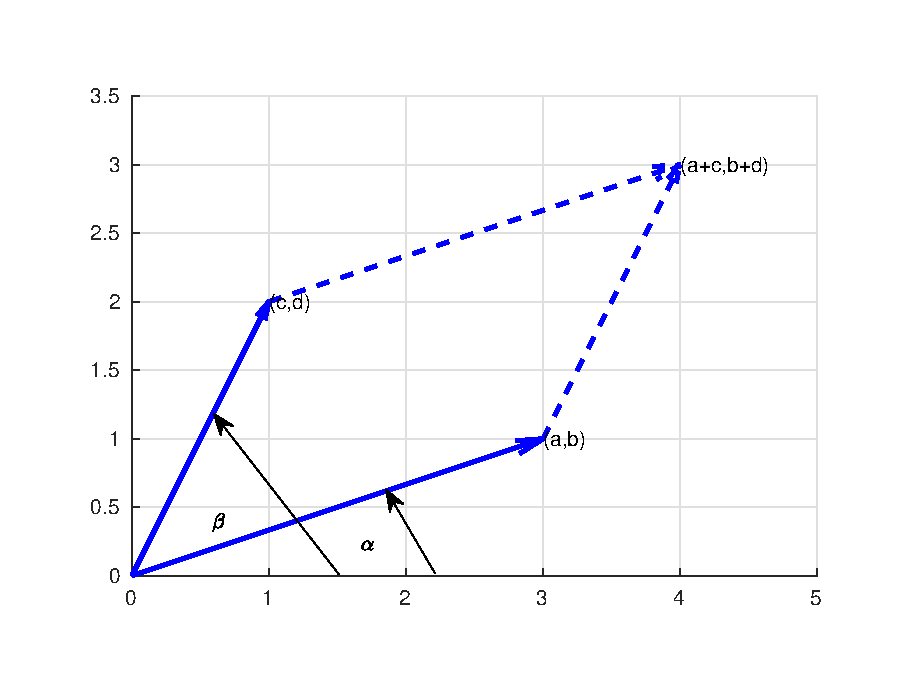
\includegraphics[width=0.75\textwidth]{fig/wyznacznik_romb}
    \caption{Geometryczna interpretacja wyznacznika macierzy $2 \times 2$.}
    \label{fig:det_romb}
\end{figure}

Można zapisać więc wzór na wyznacznik jako:
$$
    |A| = ad-bc = uv(\sin(\beta)\cos(\alpha) - \sin(\alpha)\cos(\beta)) = uv\sin(\beta-\alpha)
$$
a to jest wzór na pole równoległoboku o bokach długości $u$ i $v$
i kątem pomiędzy nimi $\beta - \alpha$.

W przypadku $n=3$ będzie to objętość równoległościanu, 
a w wyższych wymiarach odpowiednie jej uogólnienia.
%===============================================================
\subsection{Własności}
Macierz $A = [a_{ij}]$ wymiaru $n \times n$.
\begin{itemize}
    \item $|A \cdot B| = |A|\cdot|B|$
    \item $|A^{k}| = |A|^{k}$
    \item $|A^{T}| = |A|$
    \item jeśli jakiś rząd lub któraś kolumna macierzy $A$ jest 
        złożona z samych zer, wówczas wyznacznik wynosi $0$
        - odpowiada to wektorowi o długości $0$ w interpretacji
        geometrycznej
    \item przestawienie kolumny/wiersza w macierzy $A$ zmienia znak
        wyznacznika - odpowiada to zmianie kolejności wektorów W
        interpretacji geometrycznej
    \item wyznacznik macierzy posiadającej dwie identyczne kolumny/wiersze
        jest równy zeru - w interpretacji geometrycznej odpowiada to 
        dwóm identycznym wektorom, pole pomiędzy nimi jest równe $0$
    \item jeżeli któraś kolumna/rząd macierzy $A$ zostanie przemnożona
        przez pewną stałą $c$, to wyznacznik jest przemnożony przez $c$
        - w interpretacji geometrycznej odpowiada to skróceniu, 
        przemnożeniu jednego z wektorów
    \item $|cA| = c^{n}|A|$ - jest to równoważne przemnożeniu każdej 
        kolumny/wiersza przez $c$
    \item Jeżeli do dowolnej kolumny/wiersza macierzy $A$ dodamy 
        przeskalowaną (przemnożoną przez dowolną liczbę $c$) 
        kolumnę/wiersz - to wyznacznik się nie zmienia.
    \item Jeżeli dowolna kolumna/wiersz macierzy $A$ jest sumą
        dwóch składników, wówczas wyznacznik jest równy 
        sumie wyznaczników macierzy, w których kolumna ta 
        jest zamieniona tymi składnikami
\end{itemize}

%%%%%%%%%%%%%%%%%%%%%%%%%%%%%%%%%%%%%%%%%%%%%%%%%%%%%%%%%%%%%%%%
\section{Odwrotność Macierzy}
%===============================================================
\subsection{Definicja}
Macierz $A = [a_{ij}]$ wymiaru $n \times n$ - macierz kwadratowa.
Macierzą odwrotną do macierzy $A$ nazywamy taką macierz $A^{-1}$,
która spełnia warunek:
$$
    AA^{-1} = A^{-1}A = I_{n}
$$
Jeżeli macierz nie posiada odwrotności, to jej wyznacznik wynosi $0$.
Jeśli $|A| \neq 0$, to macierz odwrotna istnieje i jest wyznaczona
jednoznacznie.

Macierz odwrotną można wyznaczyć jako macierz dołączoną $adj(A)$
(transponowaną macierz dopełnień algebraicznych) podzieloną
przez wyznacznik macierzy $A$:
$$
    A^{-1} = \frac{adj(A)}{|A|}
    =
    \frac{1}{|A|}
    \begin{bmatrix} D_{11}  & D_{12}    & \cdots    & D_{1n}    \\
                    D_{21}  & D_{12}    & \cdots    & D_{2n}    \\
                    \vdots  & \vdots    & \ddots    & \vdots    \\
                    D_{n1}  & D_{n2}    & \cdots    & D_{nn}    \\
    \end{bmatrix}^{T}
$$
%===============================================================
\subsection{Własności}
Macierz $A = [a_{ij}]$ wymiaru $n \times n$.
\begin{itemize}
    \item $|A^{-1}| = |A|^{-1}$
    \item $(A^{-1})^{-1} = A$
    \item $(A^{-1})^{T} = (A^{T})^{-1}$
    \item $(AB)^{-1} = B^{-1}A^{-1}$
    \item $(\alpha A)^{-1} = \frac{1}{\alpha}A^{-1}$,
        gdzie $\alpha \in \mathbb{C} \diagup \{\mathbf{0}\}$
    \item $(A^{n})^{-1} = (A^{-1})^{n}$
\end{itemize}

\end{document}